\documentclass{article}
\usepackage{graphicx} % Required for inserting images
\usepackage{amsmath}
\title{Fourier Series Shift}
\author{Shruti Shrirang Karandikar}
\date{June 2025}

\begin{document}

\maketitle

\section{Introduction}
Fourier series are powerful mathematical tools that allow us to represent periodic functions as infinite sums of sine and cosine terms. Named after the French mathematician Jean-Baptiste Joseph Fourier (1768-1830), these series have profound applications in various fields including signal processing, physics, engineering, and data analysis.\\

At their core, Fourier series express a periodic function as a weighted sum of sinusoids (sine and cosine functions) of different frequencies. Each sinusoid contributes to the overall shape of the function, with the weights (coefficients) determining how much each frequency component contributes to the final representation. This decomposition reveals the frequency content of a signal, providing insights into its fundamental characteristics.\\

In this paper, we examine what happens to the Fourier representation when a function is transformed. These transformations include horizontal shifts (time or space delays), vertical shifts (amplitude offsets), stretching, and compression of functions. When we apply these operations to a function in the time or space domain, its Fourier representation changes in specific and predictable ways.\\

The shifting and scaling properties of Fourier series demonstrate elegant mathematical relationships. For instance, a horizontal shift in the time domain corresponds to a phase shift in the frequency domain, while stretching a function compresses its frequency representation and vice versa.\\

This paper aims to provide an accessible introduction to Fourier series transformations, focusing on the core concepts and developing an intuition about the impact of the transformations. By understanding how these basic operations affect Fourier representations, we gain powerful insights into signal analysis and processing techniques used across multiple disciplines.\\


\section{General Fourier Series Equations}

Before examining the specific case of square waves, let's recall the general equations for Fourier series. For a periodic function $f(x)$ with period $2L$, the Fourier series representation is given by:


\begin{enumerate}
    \item Synthesis Equation
    \begin{equation}
    f(x) = \frac{a_0}{2} + \sum_{n=1}^{\infty} \left[ a_n \cos\left(\frac{nx\pi}{L}\right) + b_n \sin(\frac{nx\pi}{L}) \right] 
\end{equation}


Where the coefficients are determined by the following analysis equations:

    \item Analysis Equations
    \begin{equation}
    a_0 = \frac{1}{L} \int_{-L}^{L} f(x) \, dx
    \label{a0}
    \end{equation}
    \begin{equation}
    a_n = \frac{1}{L} \int_{-L}^{L} f(x) \cos(\frac{nx\pi}{L}) \, dx, \quad n \geq 1
    \end{equation}
    \begin{equation}
    b_n = \frac{1}{L} \int_{-L}^{L} f(x) \sin(\frac{nx\pi}{L}) \, dx, \quad n \geq 1
    \label{bn}
    \end{equation}
    \end{enumerate}

\section{Square Wave}
The standard square wave function with period $2L$ and amplitude $A$ can be defined as:
\begin{equation}
    f(x) = 
\begin{cases} 
-A,     -L < x < 0 \\
A,      0 < x < L
\end{cases}
    \end{equation}

When we compute the Fourier coefficients for this square wave, we get:
\begin{eqnarray}
a_0 &=& 0 \\
a_n &=& 0 \quad \text{for all } n\\
b_n &=& 
\begin{cases} 
\frac{4A}{n\pi}, & \text{for odd } n \\
0, & \text{for even } n
\end{cases}
\end{eqnarray}

Therefore, the Fourier series for the standard square wave becomes:
\begin{equation}
    f(x) = \frac{4A}{\pi} \sum_{n=1,3,5,...}^{\infty} \frac{1}{n} \sin\left(\frac{n\pi x}{L}\right)
    \end{equation}

For the transformations we will look ar a special case:
\begin{equation}
f(x) = 
\begin{cases} 
-1, & -\pi < x < 0 \\
1, & 0 < x < \pi
\end{cases}
\end{equation}

\section{Transformations of Functions}

In this section, we explore how various transformations of a function affect its Fourier series representation. Using the square wave as our example, we'll examine four fundamental transformations: horizontal shifting, vertical shifting, stretching, and compression.

\subsection{Vertical Shifting}
    
Consider a vertical shift of 1, then the function becomes:
\begin{equation}
g(x) = 
\begin{cases} 
0, & -\pi < x < 0 \\
2, & 0 < x < \pi
\end{cases}
\end{equation}


\begin{figure}
        \centering
        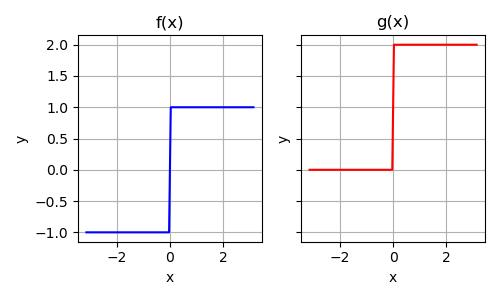
\includegraphics[width=\textwidth]{vertical_shift.jpg}
        \caption{Vertical Shifting}
        \label{fig:enter-label}
    \end{figure}

Using equation \ref{a0} to \ref{bn}, for this square wave we get:
    \begin{equation}
    a_0 = 2
    \end{equation}
    \begin{equation}
    a_n = 0
    \end{equation}
    \begin{equation}
    b_n = \frac{4}{n\pi}
    \end{equation}\\
And the Fourier series becomes:

    \begin{equation}
g(x) = 1 + \frac{4}{\pi} \sum_{n=1,3,5,...}^{\infty} \frac{1}{n} \sin\left(nx\right)
    \end{equation}\\
The average value of a Fourier series is represented by $a_0$. My original $f(x)$ ranged from
   $-1$ to $1$, so the average was $0$. This $g(x)$ ranges from $0$ to $2$, and its average is $1$. Thus, a vertical shift in the time domain affects only the average value in the frequency domain. 

\subsection{Horizontal Shifting}
Consider a horizontal shift of $\pi$, then the function becomes:
\begin{equation}
g(x) = 
\begin{cases} 
-1, & 0 < x < \pi \\
1, & \pi < x < 2\pi
\end{cases}
\end{equation}\\
\begin{figure}
    \centering
    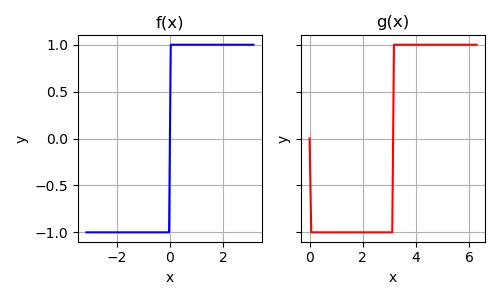
\includegraphics[width=\textwidth]{horizontal_shift.jpg}
    \caption{Horizontal Shifting}
    \label{fig:enter-label}
\end{figure}
Using equation \ref{a0} to \ref{bn}, for this square wave we get:
    \begin{equation}
    a_0 = 0
    \end{equation}
    \begin{equation}
    a_n = 0
    \end{equation}
    \begin{equation}
    b_n = \frac{-4}{n\pi}
    \end{equation}\\
And the Fourier series becomes:
\begin{equation}
g(x) = \frac{-4}{\pi} \sum_{n=1,3,5,...}^{\infty} \frac{1}{n} \sin\left(nx\right)
\end{equation}\\
We can see that $b_n$ has changed but really speaking only the sign has changed. We can incorporate this into the $\sin(nx)$ as $\sin(-nx) = \sin(\pi + nx)$. Thus a horizontal shift does not change the coefficients but results in a phase change.

\subsection{Vertical Scaling}
Consider a vertical stretch of 2, then function becomes: 
\begin{equation}
g(x) = 
\begin{cases} 
-2, & -\pi < x < 0 \\
2, & 0 < x < \pi
\end{cases}
\end{equation}\\
\begin{figure}
    \centering
    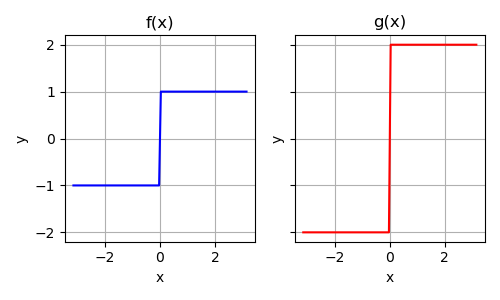
\includegraphics[width=\textwidth]{vertical_scaling.png}
    \caption{Vertical Scaling}
    \label{fig:enter-label}
\end{figure}
\begin{figure}
    \centering
    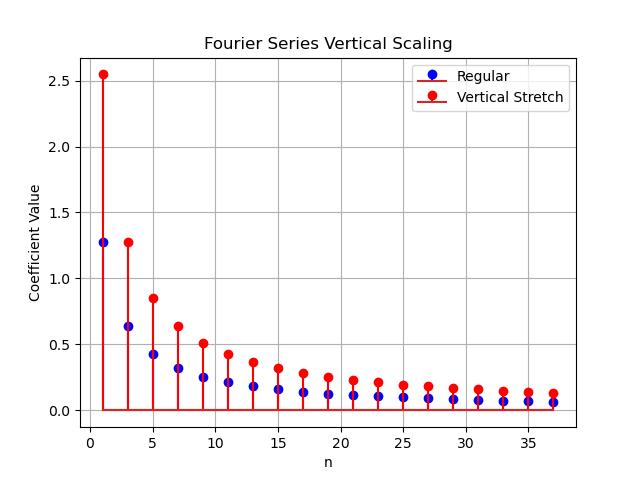
\includegraphics[width=\textwidth]{vertical_stem_stretch.jpg}
    \caption{Plotting $b_n$}
    \label{fig:enter-label}
\end{figure}
Using equation \ref{a0} to \ref{bn}, for this square wave we get:
    \begin{equation}
    a_0 = 0
    \end{equation}
    \begin{equation}
    a_n = 0
    \end{equation}
    \begin{equation}
    b_n = \frac{8}{\pi}
    \end{equation}\\
And the Fourier series becomes:
    \begin{equation}
g(x) = \frac{8}{\pi} \sum_{n=1,3,5,...}^{\infty} \frac{1}{n} \sin\left(nx\right)
    \end{equation}\\
When $g(x)$ is scaled vertically, $b_n$ is scaled by a factor of 2. Thus, the shape of the frequency spectrum remains the same while changing its magnitude.  

\subsection{Horizontal Scaling}
Consider a horizontal scale of 2, then the function becomes:
\begin{equation}
g(x) = 
\begin{cases} 
-1, & -2\pi < x < 0 \\
1, & 0 < x < 2\pi
\end{cases}
\end{equation}\\
\begin{figure}
    \centering
    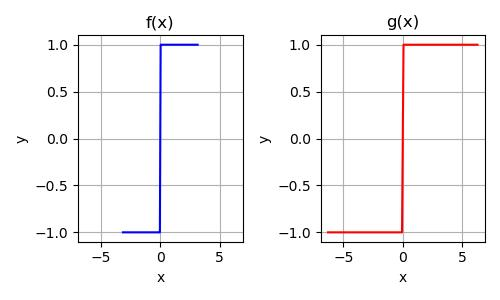
\includegraphics[width=\textwidth]{horizontal_scaling.jpg}
    \caption{Horizontal Scaling}
    \label{fig:enter-label}
\end{figure}
\begin{figure}
    \centering
    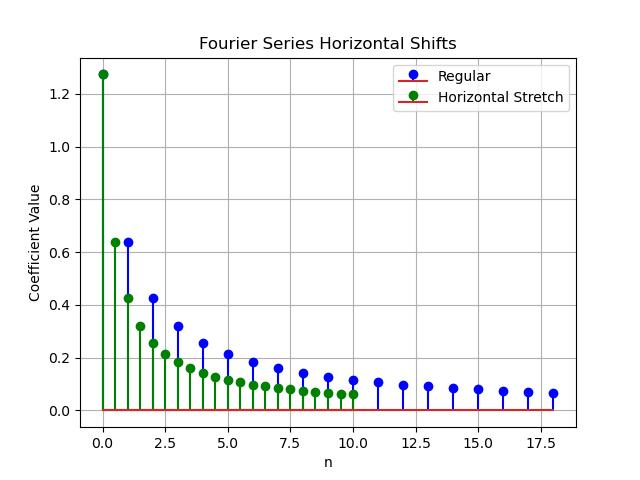
\includegraphics[width=\textwidth]{horizontal_stem_stretch.jpg}
    \caption{Plotting $b_n$}
    \label{fig:enter-label}
\end{figure}
Using equation \ref{a0} to \ref{bn}, for this square wave we get:
    \begin{equation}
    a_0 = 0
    \end{equation}
    \begin{equation}
    a_n = 0
    \end{equation}
    \begin{equation}
    b_n = \frac{4}{\pi}
    \end{equation}\\
And the Fourier series becomes:

    \begin{equation}
g(x) = \frac{4}{\pi} \sum_{n=1,3,5,...}^{\infty} \frac{1}{n} \sin\left(\frac{nx}{2}\right)
    \end{equation}\\
When $g(x)$ undergoes a horizontal scale of 2, the function is compressed horizontally. In the frequency domain, this horizontal compression causes the spectrum to expand. Specifically, if the original function has frequency components at intervals of $n$, the compressed function will have components at intervals of $n/2$. This means the harmonics appear at twice the original frequencies.\\
If $scale>1$, the function is compressed horizontally, resulting in a wider frequency spectrum.\\
If $0<scale<1$, the function is stretched horizontally, resulting in a narrower frequency spectrum.

    
\section{Generalization of Fourier Series Transformations}
In this section, we explore how the transformation principles we established for square waves can be generalized to other periodic functions. We'll examine how these transformations apply to different common functions, demonstrating the universality of these principles.

\subsection{General Principles of Transformation}
The transformation principles we've established are not limited to square waves but apply to any periodic function $f(x)$. We can repeat this for other waves and we find that its similar.

    \begin{enumerate}
    \item Triangular Wave\\
Equation of the function: 

\begin{equation}
f(x) = 
\begin{cases} 
|x|, & -\pi \leq x \leq \pi \\
\end{cases}
\end{equation}

The triangular wave with period $2L$ and amplitude $A$ has the Fourier series:

$$f(x) = \frac{8A}{\pi^2} \sum_{n=1,3,5,...}^{\infty} \frac{1}{n^2} \sin\left(\frac{n\pi x}{L}\right)$$

Applying a horizontal shift:

$$g(x) = \frac{8A}{\pi^2} \sum_{n=1,3,5,...}^{\infty} \frac{1}{n^2} \sin\left(\frac{n\pi (x-x_0)}{L}\right)$$

Applying a vertical shift:

$$g(x) + \frac{8A}{\pi^2} \sum_{n=1,3,5,...}^{\infty} \frac{1}{n^2} \sin\left(\frac{n\pi x}{L}\right)$$

Applying horizontal scaling by factor $a$:

$$g(x) = \frac{8A}{\pi^2} \sum_{n=1,3,5,...}^{\infty} \frac{1}{n^2} \sin\left(\frac{n\pi ax}{L}\right)$$

Applying vertical scaling by factor $B$:

$$g(x) = \frac{8BA}{\pi^2} \sum_{n=1,3,5,...}^{\infty} \frac{1}{n^2} \sin\left(\frac{n\pi x}{L}\right)$$

Note that while the coefficients differ from the square wave (decreasing as $1/n^2$ rather than $1/n$), the transformation principles apply identically.

    \item Sawtooth Wave\\
Equation of the function: 

\begin{equation}
f(x) = 
\begin{cases} 
\frac{x}{\pi}, & -\pi \leq x < \pi \\
f(x + 2\pi), & \text{otherwise}
\end{cases}
\end{equation}

The sawtooth wave with period $2L$ and amplitude $A$ has the Fourier series:

$$f(x) = \frac{2A}{\pi} \sum_{n=1}^{\infty} \frac{(-1)^{n+1}}{n} \sin\left(\frac{n\pi x}{L}\right)$$

When applying our transformations:\\
Horizontal shift: Phase shifts are introduced to each harmonic\\
Vertical shift: Only adds a constant term\\
Horizontal scaling: Changes the effective period and frequency spacing\\
Vertical scaling: Multiplies all coefficients by the scaling factor\\

Note that unlike the square wave, the sawtooth wave contains all harmonics, not just odd ones.
    \end{enumerate}

If I have a horizontal shift, then $g(x) = f(x-k)$. So, now $f(x-k) = g(x)$! Now I can see the general principle.

By doing a transform we can calculate $a_0$, $a_n$ and $b_n$ or we can apply to the Fourier series definition and get the same result.

And therefore, these are the formulae:
\begin{enumerate}
 \item Horizontal Shifting Formulation
    
    \begin{equation}
    f(x-x_0) = \frac{a_0}{2} + \sum_{n=1}^{\infty} \left[ a_n \cos\left(\frac{n\pi (x-x_0)}{L}\right) + b_n \sin\left(\frac{n\pi (x-x_0)}{L}\right) \right]
    \end{equation}


\item Vertical Shifting Formulation
    
    \begin{equation}
   f(x)+C = \frac{a_0+2C}{2} + \sum_{n=1}^{\infty} \left[ a_n \cos\left(\frac{n\pi x}{L}\right) + b_n \sin\left(\frac{n\pi x}{L}\right) \right]
    \end{equation}

\item Stretching and Compression Formulation

    \begin{equation}
f(ax) = \frac{a_0}{2} + \sum_{n=1}^{\infty} \left[ a_n \cos\left(\frac{n\pi ax}{L}\right) + b_n \sin\left(\frac{n\pi ax}{L}\right) \right]
    \end{equation}

\item Amplitude Scaling Formulation

    \begin{equation}
Bf(x) = \frac{Ba_0}{2} + \sum_{n=1}^{\infty} \left[ Ba_n \cos\left(\frac{n\pi x}{L}\right) + Bb_n \sin\left(\frac{n\pi x}{L}\right) \right]
    \end{equation}

\end{enumerate}

These principles remain valid regardless of the specific function being transformed.

These principles can be summarized as:

\begin{align}
\text{Horizontal Shift: affects phase but not magnitude} \\
\text{Vertical Shift: only affects the constant term } a_0 \\
\text{Horizontal Scaling: changes period and frequency spacing} \\
\text{Vertical Scaling: scales all coefficients equally}
\end{align}

\section{Conclusion}
The transformation principles we have explored throughout this paper—horizontal shifting, vertical shifting, stretching, and compression—represent fundamental operations that can be applied to any function with a valid Fourier series representation. While we used the square wave as our primary example due to its straightforward Fourier series, these principles extend universally.\\

The beauty of Fourier analysis lies in this consistency. Whether we are working with square waves, triangular waves, sawtooth functions, or arbitrary periodic signals, the mathematical relationships governing how Fourier coefficients change under transformation remain the same. A horizontal shift always introduces phase changes while preserving magnitudes. A vertical shift only affects the constant term. Horizontal scaling alters the period and frequency spacing. Vertical scaling multiplies all coefficients equally.\\

These transformations are linear transforms. Any linear operation will follow these rules-- extrapolating from this exercise, the Fourier series of a periodic function that is a linear combination of other functions will be the linear combination of the Fourier series of the composing functions.\\

\end{document}
